\documentclass{article}
\usepackage{graphicx}
\usepackage[localise=on]{xepersian}
\settextfont{XB Yas}
\begin{document}
	\عنوان{آموزش جنگو مهران تعریف}
	\عنوان‌ساز
	\صفحه‌جدید
	\فهرست‌مطالب
	\صفحه‌جدید
	\قسمت{قسمت ۵۱ نوشتن mixin های شخصی برای مدیریت بهتر کد}
		\زیرقسمت{‌\متن‌لاتین{‌Bug Fix}}
		لینک به اسم نویسنده داخل صفحه اصلی زیر مقاله ها درست کار نمیکنه چون داخل ویو کلاس یوزر خود جنگو لود میکنه ولی ما از 
		کلاس یوزر شخصی استفاده میکنیم(داخل تمپلیت ها هم به جای اشتباهی لینک شده بود و خود تمپلیت هم همه مقاله هارا نشان میداد هم 
		منتشر شده هم بایگانی) و استریپ کردن تگ ها داخل صفحه اصلی و صفحه مقالات نویسنده

		\زیرقسمت{فقط سوپر یوزر بتواند فیلد های نویسنده و وضعیت یک مقاله را مشخص کند}
		برای پیاده سازی این قابلیت از میکسین ها استفاده میکنیم هم کد تکراری کم میشه هم نگهداری اسان تر میشه.
		یک فایل \متن‌لاتین{mixins.py} داخل پوشه اپ میسازیم و یک کلاس داخل درست کنیم داخل کلاس متد dispathc را override
		 میکنیم dispatch متدی هست که ریکوست رو میگیره و یک ریسپانس برمیگردونه می خوایم بگیم اگر یوزر ریکوست سوپر یوزر بود
		 فیلدهای عادی، وضعیت و نویسنده را به فرم اضافه کن درغیر این صورت اگر نویسنده بود فقط فیلد های عادی رو اضافه کن و
		 در اخر اگر هیچ یک نبود صفحه را نمایش نده(ارور بده بهش)
		 \begin{figure}[h!]
		 	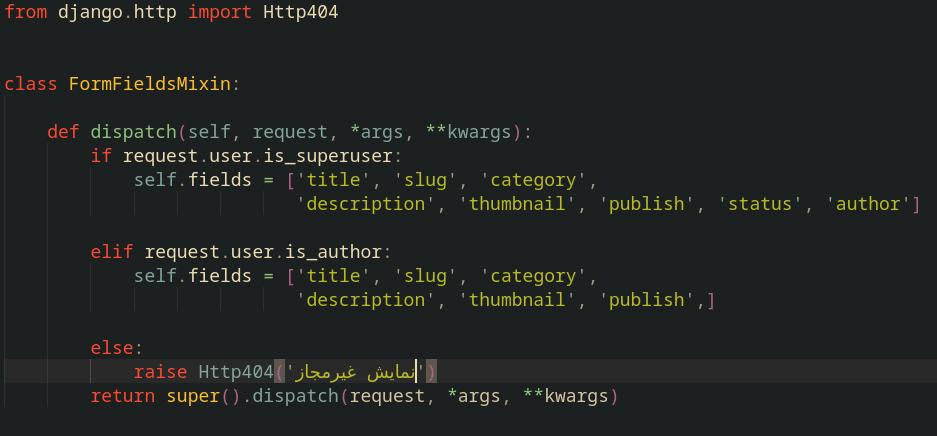
\includegraphics[width=\linewidth]{mehran-tarif-course-code-pic/FormFieldMixinPic.jpg}
		 \end{figure}
		 میکسین را در فایل \متن‌لاتین{views.py} ایمپورت میکنیم و کلاس مربوط(ساخت مقاله) ازش ارث بری میکنه
		 
		 داخل فایل تمپلیت هم فیلد های نویسنده و وضعیت که بهشون استایل دادیم داخل یک شرط قرار بگیره که تنها وقتی که کاربر
		 سوپر یوزر هست نمایش داده بشه
	
		\زیرقسمت{فیلد نویسنده به صورت پیشفرض برای نویسنده مقدار داشته باشه}
			چون نویسنده نمیتونه فیلد های نویسنده و وضعیت یک مقاله را تعیین کند میخواهیم زمانی که یک مقاله اضافه کرد اون مقاله
			به صورت دیفالت نویسندش بشه همون نویسنده‌ای که مقاله را نوشه و وضعیت هم draft باشه به صورت خودکار برای این کار از
			از یک میکسین و یک متد \متن‌لاتین{form valid} استفاده میکنیم و مشخص میکنیم اگه کاربر نویسنده عادی بود به صورت خود 
			کار نویسنده را برابر نویسنده مقاله قرار بده و از وضعیت draft استفاده کن بعد از میکسین داخل ویو مربوطه استفاده 
			میکنیم 
			
			برای اینکه بتونیم مقدار فیلد هارو داخل فرم تغییر بدیم از \متن‌لاتین{commit=False} استفاده میکنیم. 
		
		\begin{figure}[h!]
			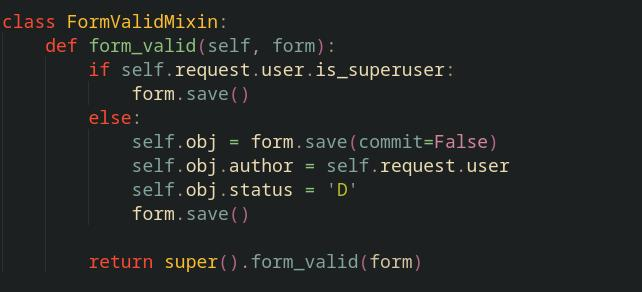
\includegraphics[width=\linewidth]{mehran-tarif-course-code-pic/FormValidMixinPic.jpg}
		\end{figure}
	
	\قسمت{قسمت۵۲ ساخت ویو آپدیت}
	\زیرقسمت{پیاده‌سازی}
		مثل همون ویو کریت هست ولی بجای create از update ارث بری میکنه(امپورت بشه) به یو ار ال ها اضافه بشه داخل یو ار ال از
		 \متن‌لاتین{primary key} استفاده کنیم و داخل تمپلیت ها هم از لینک روی اسم مقاله استفاده کنیم (چجوری ایدی پاس بدیم به یو ار ال داخل 
		 تمپلیت) 
	
	\زیرقسمت{رفع باگ}
	 کاربران میتواند با استفاده از ایدی مقاله داخل یو ار ال مقاله های پابلیشو درفت کنندبا تغییر اون یا مقاله های کس دیگه ای رو تغییر بدن
	 باید یه دسترسی داشته باشیم که هر کاربر فقط بتونه مقاله های خودشو تغییر بده اگر سوپر یوزر نبود ولی اگر سوپر یوزر بود مقاله های بقیه هم
	 بتونه تغییر بده\\
	 \زیرزیرقسمت{کد نویسی}
	 \شروع{شمارش}
	 	\فقره یدونه میکسین جدید میسازیم و از متد dispatch استفاده میکنیم
	 	\فقره با استفاده از متد \متن‌لاتین{get\_object\_or\_404} مقاله را از دیتابیس میخوانیم
	 	\فقره نویسنده مقاله را با یوزر ریکوست چک میکنیم 
	 	\فقره شروط را اعمال میکنیم
	 	
	 	\پایان{شمارش}
	 	داخل ویو از این میکسین بجا \متن‌لاتین{LoginRequired} استفاده میکنیم چون مطمئن هستیم دیگه کاربر لاگین هست
	 \زیرقسمت{رفع باگ۲}
	 کاربران عادی متوانند با تغییر دادن مقاله ی منتشر شده وضعیت مقاله را به درفت عوض کند میخوایم فقط بتوانند مقاله های درفت را تغییر
	 بدهند\\
	 \زیرزیرقسمت{کدنویسی}
	 	داخل متد dispathch در میکسین شرطمون رو اینجوری مینویسیم که کاربر عادی باشد و مقاله درفت باشه یا کاربر سوپر یوزر باشه و داخل
	 	تمپلیت هم فقط نام مقاله هایی لینک شده باشند که وضعیت درفت دارند یا کاربر سوپر یوزر باشد.
	 	
	 \قسمت{قسمت ۵۳ ساخت ویو حذف مقالات و میکسین دسترسی مدیران}
	 جنگو دیلیت ویو داکیومنتس از خود مثال داکیومنت استفاده میکنیم بخش ریورس لیزی مارو ببره به صفحه مقالات داخل پنل ادمین،‌ یو ار ال 
	 اضافه کنیم، داخل صفحه مقالات یه بدج اضافه بشه برای حذف ولی فقط برای سوپر یوزر، یدونه میکسین هم برای دیلیت اکسس(سوپریوزر اکسس) میسازیم
	 
	 \قسمت{قسمت ۵۴ ساخت ویو لاگ اوت}
	 از ادمین اصلی نوبار بالا کپی میکنیم دانلود ایکون مجانی لاگ اوت از awesome تمپلیت به صورت پیشفرض از awesome استفاده میکنه (مجانی هاش)
	 ان کامنت کردن لاگ اوت داخل یو از ال ، لینک به ویو لاگ اوت داخل تمپلیت، اسم تمپلیت لاگ اوت جنگو و محتویاتشو کپی میکنیم برای اورراید کردن 
	 داخل اپ خودمون، روش دوم داخل ستینگ این متغیر رو ست میکنیم \متن‌لاتین{LOGOUT\_REDIRECT\_URL='account:login'} 
	 \زیرقسمت{رفع باگ} 
	  اگر نویسنده هیچ مقاله ای نداشت لیست خالی نشون نده بگه کاربر هیچ مقاله ای ندارد با ایف ابحکت لیست و الس و اچ ۳
	 
	 
	 \قسمت{قسمت ۵۵ اکتیو منو و حذف مقاله از بخش ویراش}
	 استایل سفید افزودن مقاله و بخش های دیگه داخل پنل ادمین، \متن‌لاتین{request.resolver\_match} اطلاعات بیشتری از ریکوست میده
	 داخل اون نو باره گوشه کلاس اکتیو میاد سفید میکنه یک شرط با\\
	  \{\{\متن‌لاتین{request.resolver\_match.url\_name}\}\} مینویسیم یا اینکه با تمپلیت تگ بنویسیمش(اینو چک کن)\\
	  \زیرقسمت{حذف مقاله در قسمت ویرایش}
	  داخل تمپلیت یدونه شرط میذاریم که اگر کاربر سوپر یوزر بود و مقاله پی کی داشت (از ریزالور استفاده میکنیم که مطمئن بشیم داخل 
	  اپدیت هستیم نه کیریت)
	  \زیرقسمت{چجوری \متن‌لاتین{template tags} های خودمون بسازیم}
	  	\شروع{شمارش}
	  		\فقره داخل اپ یدونه دایرکتوری میسازیم به اسم \متن‌لاتین{templatetags}
	  		\فقره فایل تمپلیت تگ مثلا \متن‌لاتین{basetags.py} و اینیت داخلش میسازیم
	  		\فقره از جنگو تمپلیت رو ایمپورت میکنیم
	  		\فقره تمپلیت رو رجیستر میکنیم \متن‌لاتین{register = template.Library()}
			\فقره متد تمپلیت تگ رو با فایل اچ تی ام الش رجیستر میکنیم \متن‌لاتین{register.inclusion\_tag('file.html')}
			\فقره یک متد مینویسم با پارامتر های \متن‌لاتین{request, link\_name, content}
			

	  		\فقره خروجی متد همون ورودی هاش هست به اضافه \متن‌لاتین{link} که اسم لینک هست یک استرینگ فرمت شده مثلا \متن‌لاتین{account:home}
	  		\فقره تمپلیت مربوطه رو میسازیم 
	  		


	  	\پایان{شمارش}

		\زیرقسمت{چجوری منوی اکتیو رو فعال کنیم داخل ساید بار}
			یعنی اگر لیست مقالات انتخاب شد اون سفید باشه اگه افزودن مقاله جدید انتخاب شد اون سفید باشه و اگر رفتیم برای ویرایش هیچ کدام
			سفید نباشه
			\پاراگراف{راه اول} این هست که با استفاده از if و \متن‌لاتین{request.resolver\_match} پیاده سازیش کنیم مشکل این روش اینکه که
			کد تمپلیت شلوغ میشه 
			\پاراگراف{روش دوم(بهتر)} بیایم از تمپلیت تگ ها استفاده کنیم، یدونه تمپلیت تگ تعریف کنیم و بعد از اون استفاده کنیم
			
	\قسمت{قسمت ۵۶ ساخت پیشنمایش مقاله های پیشنویس در پنل مدیریت}
		\شروع{شمارش}
			\فقره یک ویو مثل ارتیکل دیتیل واسش میسازیم بجای سلاگ از پرایمری کی استفاده میکنیم و کوئری رو هم عوض میکنیم
			\فقره داخل یو ار ال هم ایمپورت میکنیم
			\فقره یک محدودیت باشه که فقط برای نویسنده و سوپر یوزر قابل نمایش باشه
			\فقره یک بدج براش داخل هوم درست کنیم
			
		\پایان{شمارش}
	
	\قسمت{قسمت ۵۷ افزایش وضعیت مقالات}
		حالت i مخواستیم از p استفاده کنیم یعنی pendding ولی چون واسه پابلیش بود دیگه نمیشد این حالتی هست که مقاله رفت برای چک سوپریوزر
		و دیگه نویسنده نمیتونه ادیتش کنه حالت b یعنی back حالتی هست که یعنی سوپریوزر چک کرده و ایراد گرفته ازش دوباره مقاله میشه مثل حالت
		پیشنویس(میشه طراحی کرد که یک متن هم اونجا بنویسه سوپر یوزر)
		\شروع{شمارش}
			\فقره اضافه کردن حالت ها به مدل
			\فقره تصحیح میکسین که کاربر هم بتونه به b دسترسی داشته باشه هم d 
			\فقره داخل ویو هوم ادمین هم کار مرحله قبل رو تکرار میکنیم ولی اینجا لیست نداریم از فیلتر \متن‌لاتین{make\_list} استفاده میکنیم
			\فقره بدج برای حالت های i و b بسازیم 
			\فقره در حالت i اگر یوزر سوپر یوزر بود لینک پیشنمایش رو باید نشون بدیم
			\فقره 
		\پایان{شمارش}
		
	\قسمت{قسمت ۵۸ نمایش مقالات اشتراک ویژه}
		\زیرقسمت{رفع باگ} وقتی تمپلیت تگ هارو درست میکردیم کلاس های ایکون هارو ندادیم اینو باید توی تمپلیت تگ تعریف کنیم و داخل تمپلیت
		تمپلیت تگ و خود سایت پیاده سازیش کنیم
		\زیرقسمت{پیاده سازی مقالات ویژه}
			به مدلمون یک فیلد بولین ایز اسپشیال درست میکنیم با دیفالت فالس و وربس نیم مقالات ویژه میک مایگریشن و مایگریت، داخل پنل ادمین
			جنگو هم این فیلد رو برای مقاله ها نشون بده، داخل پنل ادمین خودمون داخل فیلدی که با میکسین ها میسازیم این قابلیت رو بدیم 
			که هم نویسنده مشخص کنه این مقاله ویژه هست یا نه هم سوپر یوزر (اینجوری انتخاب نهایی با سوپریوزر هست)، داخل تمپلیت ادمین
			خودمون به اون تمپلیت کریت هم اضافه بشه، داخل تمپلیت اصلی وبسایت شرط میذاریم برای مقالات ویژه که به همه نشون نده
			شرط تو در تو فقط به کسایی که لاگین هستند و سپشیال یوزر هستند یا اینکه نویسنده همین مقاله هستند یا سوپر یوزر هستند نمایش بده 
			در غیر این صورت یک پیام بده که باید اشتراک تهیه کنید ، نمایش این فیلد ایز اسپشیال داخل جدول صفحه ادمین خودمون از ایکون های 
			فونت اسوم اسفاده کنه اگه ویژه بود یک تیک سبز (اف ای اف ای-چک-سیرکل) در غیر اینصورت علامت منفی نشون بده 
			(اف ای اف ای-ماینس-سیرکل)
\end{document}